\section{Divergenca glede na gostoto verjetnosti}

Divergenca ima lahko več pomenov. V analizi se ta pojem uporablja pri obravnavanju zaporedij in vrst (takrat govorimo o konvergenci in divergenci zaporedja oz. vrste). V tem poglavju bomo predstavili še drugi pomen divergence.

\subsection{Definicija divergence}

Najprej navedimo motivacijski zgled za uporabo divergence.

\begin{zgled}
	V podjetju s proizvodnjo na tekočem traku nas zadolžijo za oskrbo tekočega traku. Naša naloga je, da sporočimo napako, ko jo zaznamo. Napake lahko zaznamo z odstopanjem izhodnih podatkov (npr. temperatura, vibracije, glasnost, itd.).

	Nastane problem: kako sploh primerjati trenutne podatke z optimalnimi in kdaj je odstopanje podatkov dovolj veliko? Potrebujemo metodo, s pomočjo katere bomo lahko primerjali razliko med dvema množicama podatkov. Poleg tega moramo z zagotovostjo trditi, da je prišlo do napake. Pomagamo si z divergenco.
\end{zgled}

Divergenca je torej merilo za razliko med dvema statističnima vzorcema (vzorca si lahko predstavljamo kot dve porazdelitvi). Navedimo formalno definicijo.

\begin{definicija}
	Naj bo $S$ prostor vseh verjetnostnih porazdelitev na istem definicijskem območju (tj. porazdelitve z istimi nosilci - na istem območju niso enake 0). \textbf{Divergenca} na $S$ je funkcija $D(\cdot \| \cdot): S \times S \rightarrow \mathbb{R}$, tako da velja:
	\begin{enumerate}
		\item $D(p \| q) \geq 0$ za vsaka $p, q \in S$,
		\item $D(p \| q) = 0 \Leftrightarrow p = q$.
	\end{enumerate}
	\textbf{Dualna divergenca} $D^\ast$ je definirana kot $D^\ast(p \| q) = D(q \| p)$.
\end{definicija}

Divergenca ni nujno simetrična in zanjo ne velja trikotniška neenakost, zato ne moremo enačiti pojmov divergenca in metrika.



\subsection{Divergenca univariatnih porazdelitev}

Definiranih je več različnih divergenc. Vsaka divegenca ima neke koristne lastnosti (npr. ena divergenca je bolj občutljiva glede na srednje vrednosti porazdelitev, tj. bo velika, ko se bodo srednje vrednosti razlikovale; spet druga divergenca je bolj občutljiva na varianco porazdelitev).

Renyi divergenci se bomo posvetili v naslednjem poglavju. Brez dokazov, da je to res divergenca, navedimo še nekaj ostalih primerov divergenc. Navedimo samo formule za zvezne spremenljivke, saj je formula za diskretne spremenljivke analogna (namesto integrala uporabimo vsoto).

\begin{zgled}
	\leavevmode
	\begin{enumerate}
		\item \textbf{Kullback-Leiblerjeva divergenca}:
		\begin{equation}
			D_{KL}(p \| q) = \int_\Omega p(x) \cdot \log\Big(\frac{p(x)}{q(x)}\Big) \  dx,
		\end{equation}
		kjer sta $p$ in $q$ porazdelitvi z definicijskim območjem $\Omega$.
		\item \textbf{f-divergenca}:
		To je družina divergenc, generirana s funkcijami $f$, za katere velja:
		\begin{itemize}
			\item $f$ konveksna na $\mathbb{R}^+$,
			\item $f(1) = 0$.
		\end{itemize}
		Elementi te družine so oblike:
		\begin{equation}
			D_f(p \| q) = \int_\Omega p(x) \cdot f\Big(\frac{p(x)}{q(x)}\Big) \  dx,
		\end{equation}
		kjer sta $p$ in $q$ porazdelitvi definirani na definicijskem območju $\Omega$.
		\item \textbf{Hellingerjeva distanca}:
		\begin{equation}
			H^2(p, q) = 2 \int_\Omega \Big(\sqrt{p(x)} - \sqrt{q(x)}\Big)^2 \  dx,
		\end{equation}
		kjer sta $p$ in $q$ porazdelitvi definirani na definicijskem območju $\Omega$.
	\end{enumerate}
\end{zgled}

\subsection{Renyi divergenca}

Nekoliko podrobneje oglejmo \textbf{Renyi divergenco}. Omejili se bomo le na zvezne spremenljivke, saj je definicija za diskretne analogna.


\begin{definicija}
	Naj bosta $P$ in $Q$ porazdelitvi z definicijskim območjem $\Omega$, $p$ in $q$ po vrsti gostoti verjetnosti porazdelitev $P$ in $Q$ ter $\alpha > 0$, $\alpha \neq 1$. Tedaj je \textbf{Renyi divergenca} definirana kot:
	\begin{equation}
		D_{\alpha}(P \| Q)=\frac{1}{\alpha-1} \cdot \log \int_{\Omega} \Big(p(x)\Big)^{\alpha}\Big(q(x)\Big)^{1-\alpha}\  dx.
	\end{equation}
\end{definicija}

Dokazati moramo naslednji izrek:

\begin{izrek}
	Renyi divergenca je divergenca.
\end{izrek}

\begin{proof}
	Naj bo $S$ prostor gostot verjetnosti.
	Dokazati moramo:
	\begin{enumerate}
		\item $D(p \| q) \geq 0$ za vsaka $p, q \in S$,
		\item $D(p \| q) = 0 \Leftrightarrow p = q$.
	\end{enumerate}
	Najprej dokažimo, da je Renyi divergenca vedno pozitivna. Namesto $p(x)$ in $q(x)$ pišimo kar $p$ in $q$. Dokazati moramo:
	\begin{equation}
		\label{neenakost}
		\frac{1}{\alpha - 1}\log \int_\Omega p^\alpha q^{1-\alpha} \  dx \geq 0.
	\end{equation}
	Ločimo primere:
	\begin{itemize}
		\item $\alpha > 1$: ker je prvi faktor v neenakosti \ref{neenakost} pozitiven za $\alpha > 1$, je ekvivalentno dokazati, da
		\begin{equation*}
			\log \int_\Omega p^\alpha q^{1-\alpha}  dx \geq 0
		\end{equation*}
		oziroma
		\begin{equation*}
			\int_\Omega p^\alpha q^{1-\alpha}  dx \geq 1
		\end{equation*}
		oziroma
		\begin{equation*}
			\int_\Omega \Big(\frac{p}{q}\Big)^\alpha q \  dx \geq 1.
		\end{equation*}
		Uporabimo Jensenovo neenakost za konveksno funkcijo $\phi$:
		\begin{equation*}
			\phi(\int f(x) dx) \leq \int (\phi \circ f) (x) dx,
		\end{equation*}
		kjer izberemo funkcijo $\phi(t) = t^\alpha$:
		\begin{equation*}
			\int_\Omega \Big(\frac{p}{q}\Big)^\alpha q \  dx \geq \Big(\int_\Omega \frac{p}{q} q dx\Big)^\alpha = \Big(\int p dx\Big)^\alpha = 1,
		\end{equation*}
		kjer smo upoštevali, da je $\int_\Omega p dx = 1$ po definiciji gostote verjetnosti.
		\item $0 < \alpha < 1$: ker je prvi faktor v neenakosti \ref{neenakost} negativen za $0 < \alpha < 1$, je ekvivalentno dokazati, da
		\begin{equation*}
			\log \int_\Omega p^\alpha q^{1-\alpha}  dx \leq 0
		\end{equation*}
		oziroma
		\begin{equation*}
			0 < \int_\Omega p^\alpha q^{1-\alpha}  dx \leq 1
		\end{equation*}
		oziroma
		\begin{equation*}
			0 <\int_\Omega \Big(\frac{q}{p}\Big)^{1-\alpha} p \  dx \leq 1.
		\end{equation*}
		Uporabimo Jensenovo neenakost za konkavno funkcijo $\phi$:
		\begin{equation*}
			\phi(\int f(x) dx) \geq \int (\phi \circ f) (x) dx,
		\end{equation*}
		kjer izberemo funkcijo $\phi(t) = t^{1-\alpha}$:
		\begin{equation*}
			\int_\Omega \Big(\frac{q}{p}\Big)^{1-\alpha} p \  dx \leq \Big(\int_\Omega \frac{q}{p} p \ dx\Big)^{1-\alpha} = \int_\Omega q \ dx = 1,
		\end{equation*}
		kjer smo upoštevali, je $\int_\Omega q dx = 1$ po definiciji gostote verjetnosti.
	\end{itemize}
	Dokažimo še drugo točko, torej
	\begin{equation}\label{eq-ekvivalenca-renyi}
		\frac{1}{\alpha - 1}\log \int_\Omega p^\alpha q^{1-\alpha} \  dx = 0 \Leftrightarrow p = q.
	\end{equation}
	Najprej dokažimo implikacijo iz desne proti levi ($\Leftarrow$):
	\begin{equation*}
		\frac{1}{\alpha - 1}\log\int_\Omega \Big(\frac{p}{p}\Big)^\alpha p \  dx = \frac{1}{\alpha - 1}\log\int_\Omega p \  dx = \frac{1}{\alpha - 1}\log 1 = 0.
	\end{equation*}
	V drugo smer ($\Rightarrow$) naredimo kratek premislek. Izraz na levi strani ekvivalence \eqref{eq-ekvivalenca-renyi} bo enak $0$, ko:
	\begin{enumerate}
		\item $\alpha = 0$, kar je v protislovju s predpostavko, da je $\alpha > 0$,
		\item $p = q$, saj bo takrat \ \  $\log\int_\Omega p \ dx = \log 1 = 0$.
	\end{enumerate}
	Zadnja implikacija je dokazana površno, saj bi se lahko zgodilo tudi, da implikacija ($\Rightarrow$) iz 2. točke velja, če $p \neq q$. Zaključimo, da se to zaradi lastnosti gostot verjetnosti ne more zgoditi.
\end{proof}

Renyi divergenca ni definirana v $\alpha = 1$, a v tej točki poznamo njeno vrednost:

\begin{izrek}\label{div_v_1}
	Naj bo $D_\alpha(P \| Q)$ Renyi divergenca porazdelitev $P$ in $Q$. Tedaj velja:
	\begin{equation}
		\lim_{\alpha \rightarrow 1} D_\alpha(P \| Q) = \int_\Omega p(x) \cdot \log\Big(\frac{p(x)}{q(x)}\Big) \  dx,
	\end{equation}
	kjer je izraz na desni ravno \textbf{Kullback-Leiblerjeva} divergenca porazdelitev $P$ in $Q$, tj.
	\begin{equation}
		\lim_{\alpha \rightarrow 1} D_\alpha(P \| Q) = D_{KL} (P \| Q).
	\end{equation}
\end{izrek}

Dokažimo izrek \ref{div_v_1}:

\begin{proof}
	Izračunajmo limito $D_\alpha(P \| Q)$, ko gre $\alpha$ proti $1$.
	\begin{equation*}
		\lim_{\alpha \rightarrow 1} \frac{\log \int p(x)^{\alpha}q(x)^{1-\alpha}\  dx}{\alpha-1} = \mathquotes{\frac{0}{0}},
	\end{equation*}
	zato lahko uporabimo L'Hospitalovo pravilo:
	\begin{equation*}
		\lim_{x \rightarrow a} \frac{f(x)}{g(x)} = \lim_{x \rightarrow a} \frac{f'(x)}{g'(x)}.
	\end{equation*}
	Posebej izračunajmo odvoda števca in imenovalca. Odvod imenovalca je trivialen: $(\alpha - 1)' = 1$. Odvajajmo še števec:
	\begin{align*}
		&\frac{d}{d\alpha}\Big( \log \int_\Omega p(x)^{\alpha}q(x)^{1-\alpha}\  dx\Big) = \frac{1}{\int_\Omega p(x)^{\alpha}q(x)^{1-\alpha}\  dx} \quad  \frac{d}{d\alpha}\int_\Omega p(x)^{\alpha}q(x)^{1-\alpha}\  dx \overset{(\ast)}{=} \\ &\overset{(\ast)}{=} \frac{1}{\int_\Omega p(x)^{\alpha}q(x)^{1-\alpha}\  dx} \quad \int_\Omega \frac{\partial}{\partial\alpha}\Big(p(x)^{\alpha}q(x)^{1-\alpha}\  dx\Big) = \\ &= \frac{1}{\int_\Omega p(x)^{\alpha}q(x)^{1-\alpha}\  dx} \quad \int_\Omega \Big(p(x)^\alpha \cdot \log p(x) \cdot q(x)^{1 - \alpha} - p(x)^\alpha \cdot q(x)^{1 - \alpha} \cdot \log q(x)\Big)dx = \\ &= \frac{1}{\int_\Omega p(x)^{\alpha}q(x)^{1-\alpha}\  dx} \quad \int_\Omega p(x)^\alpha \cdot q(x)^{1 - \alpha} \cdot \log \frac{p(x)}{q(x)} \ \  dx,
	\end{align*}
	kjer smo pri $(\ast)$ upoštevali, da je $F(\alpha) = p(x)^\alpha \cdot q(x)^{1 - \alpha}$ zvezna funkcija. Če izračunamo limito kvocienta odvodov, dobimo:
	\begin{equation*}
		\lim_{\alpha \rightarrow 1} \frac{\int_\Omega p(x)^\alpha \cdot q(x)^{1 - \alpha} \cdot \log \frac{p(x)}{q(x)} \ \  dx}{\int_\Omega p(x)^{\alpha}q(x)^{1-\alpha}\  dx} = \frac{1}{\int_\Omega p(x)\  dx} \ \int_\Omega p(x) \cdot \log \frac{p(x)}{q(x)} \ \  dx.
	\end{equation*}
	Če upoštevamo, da $\int_\Omega p(x) \ \ dx = 1$, dobimo:
	\begin{equation*}
		\int_\Omega p(x) \cdot \log \frac{p(x)}{q(x)} \ \  dx
	\end{equation*}
	kar je po definiciji ravno Kullback-Leiblerjeva divergenca.
\end{proof}



\subsection{Renyi divergenca normalnih porazdelitev}

Kot zgled si poglejmo izračun Renyi divergence za nekaj normalnih porazdelitev. Podajmo jih z enačbami:

\begin{equation}\label{norm_porazd}
	\begin{aligned}
		\N_1^{0,1}(x) &= \frac{1}{\sqrt{2\pi}}\cdot e^{-\frac{x^2}{2}} \\
		\N_2^{5,1}(x) &= \frac{1}{\sqrt{2\pi}}\cdot e^{-\frac{(x-5)^2}{2}} \\
		\N_3^{0,5}(x) &= \frac{1}{5\sqrt{2\pi}}\cdot e^{-\frac{x^2}{50}} \\
		\N_4^{0,10}(x) &= \frac{1}{10\sqrt{2\pi}}\cdot e^{-\frac{x^2}{200}}.
	\end{aligned}
\end{equation}

kjer je $\N_i^{\mu_i, \sigma_i}$ gostota verjetnosti porazdelitve $P_i$. Za predstavo si oglejmo še grafe teh verjetnostnih porazdelitev:

\begin{figure}[!ht]
	\centering
	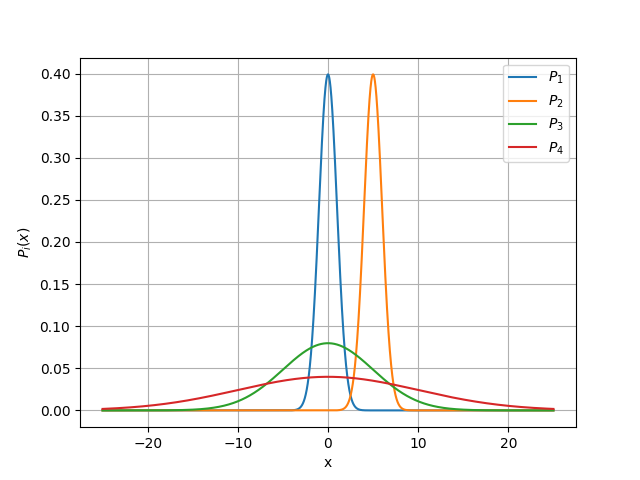
\includegraphics[scale=0.8]{normalne4}
	\caption{Normalne porazdelitve.}
\end{figure}

Brez simbolnega računanja si poglejmo divergenco med normalnimi porazdelitvami \eqref{norm_porazd}.

\begin{figure}[!ht]
	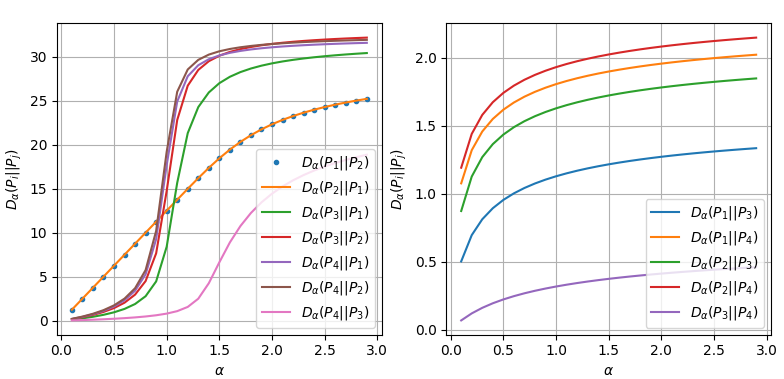
\includegraphics[scale=0.8]{divnorm}
	\caption{Divergence normalnih porazdelitev.}
	\label{divergence}
\end{figure}
\pagebreak
Na podlagi izračunov omenimo ugotovitvi:
\begin{enumerate}
	\item Opazimo, da bo vrednost Renyi divergence zelo velika, če bo varianca prve porazdelitve večja kot varianca druge porazdelitve in majhna, če bo varianca prve porazdelitve manjša kot varianca druge porazdelitve.
	\item Če je varianca porazdelitev $P_1$ in $P_2$ enaka, je Renyi divergenca simetrična, t.j. 
	\begin{equation*}
		D(P_1 \| P_2) = D^{\ast}(P_1 \| P_2) = D(P_2 \| P_1).
	\end{equation*}
\end{enumerate}

Če lahko sklepamo na podlagi Renyi divergence normalnih porazdelitev smo ugotovili, da na Renyi divergenco zelo vpliva razmerje med variancama prve in druge porazdelitve. Zaradi tega je lahko razlika med vrednostjo Renyi divergence in vrednostjo dualne Renyi divergence zelo velika.

Brez dokaza omenimo še, da translacija sistema ne vpliva na izračun Renyi divergence normalnih porazdelitev, to pomeni:
\begin{equation}
	D_\alpha\Big(\N^{\mu_1, \sigma_1}(x) \| \N^{\mu_2, \sigma_2}(x)\Big) = D_\alpha\Big(\N^{\mu_1, \sigma_1}(x - a) \| \N^{\mu_2, \sigma_2}(x - a)\Big),
\end{equation}
kjer je $a \in \mathbb{R}$.

\begin{opomba}
	Izračun divergenc in izris grafov sta bila narejena s programskim jezikom \texttt{Python3}.
\end{opomba}

\subsection{Numerično računanje Renyi divergence}

Kljub temu, da v definiciji divergence zahtevamo, da imata porazdelitvi ista nosilca oz. sta na istih območjih neničelni, se to v praksi pogostokrat ne obnese.

Prva težava je, da bi mogoče hoteli primerjati tudi porazdelitve, ki nimajo istih nosilcev. Vsako porazdelitev lahko razširimo na $\RR$ tako, da ji povsod, kjer ta ni definirana, priredimo vrednost 0. S tem sicer dobimo porazdelitvi z istim difinicijskim območjem, a nimata istih nosilcev. Seveda pa se poraja vprašanje, ali je sploh smiselno primerjati porazelitvi z različnima nosilcema? Na primer, ali je smiselno primerjati uniformno porazdelitev na intervalu $[0, 1]$ z uniformno porazdelitvijo na intervalu $[2, 3]$? Bralec naj to presodi sam.

Drugo težavo malce bolj analizirajmo, saj se pojavi tudi, ko imata porazdelitvi ista nosilca. Kot primer vzemimo normalni porazdelitvi. Gostota verjetnosti normalne porazdelitve je funkcija $\RR \rightarrow \RR^+$, torej bi morali pri Renyi divergenci dveh normalnih porazdelitev vedno dobiti rezultat v množici realnih števil.

Naj bosta $p$ in $q$ gostoti verjetnosti poljubnih realnih funkcij. Problem nastane v repih normalnih porazdelitev. Kljub temu, da je $p(x) > 0$ in $q(x) > 0$ za vsak $x \in \RR$, pride do numeričnih težav (deljenje z ničlo). Zakaj? Pride do podkoračitve (v neki točki nam računalnik zaokroži vrednost $p(x)$ na 0). Vpeljimo pojem konstante numerične ločljivosti.

\begin{definicija}
    \textbf{Konstanta numerične ločljivosti} je najmanjše pozitivno število, ki ga operacijski sistem še ne zaokroži na 0 (t.j. v operacijskem sistemu najmanjše predstavljivo število).
\end{definicija}

\begin{zgled}
    V 64-bitnem operacijskem sistemu je konstanta numerične ločljivosti enaka \\$\epsilon = 2,220446049250313 \cdot 10^{-16}$. Torej bodo vsa števila med 0 in $\epsilon$ zaokrožena na 0.
\end{zgled}

Predpostavimo, da operiramo s 64-bitni sistemom. Naj bo od zdaj naprej \begin{equation*}
    \epsilon = 2,220446049250313 \cdot 10^{-16}.
\end{equation*}

Torej, normalna porazdelitev $p$ bo neničelna le na intervalu $[x_1, x_2]$, kjer sta $x_1$ in $x_2$ rešitvi enačbe $p(x) = \epsilon$, za število $a$ na komplementu tega intervala pa bo $p(a)=0$. Analogno sklepamo za normalno porazdelitev $q$.

Zaradi takšnega zaokroževanja pride pri izračunu Renyi divergence do deljenja s številom 0. Spomnimo se formule za izračun Renyi divergence:
\begin{equation}
D_\alpha(p \| q) =
\begin{cases}
    \frac{1}{\alpha-1} \log \int_{\Omega} p(x)^{\alpha}q(x)^{1-\alpha}  dx&, \quad \alpha \neq 1 \\
    \quad \int_{\Omega} p(x) \log \frac{p(x)}{q(x)} dx&, \quad \alpha = 1
\end{cases}
\end{equation}
Najprej obravnavajmo težave pri $\alpha \neq 1$. Pride do deljenja z ničlo, ko je $q(x) = 0$ za nek $x$, ker je 
\begin{equation}
    q(x)^{1-\alpha} = q(x)\cdot\Big(\frac{1}{q(x)}\Big)^\alpha.
\end{equation}
Temu problemu se izognemo tako, da definiramo:
\begin{itemize}
    \item $\frac{0}{0}=0$,
	\item $\frac{a}{0}=\infty$ \ za $a>0$,
	\item $\log\infty = \infty$.
\end{itemize}
Če se torej zgodi, da so obe gostoti hkrati 0, ni težav. Ampak v trenutku, ko je $q(x) = 0$ in $p(x) \neq 0$, bo $D_\alpha(p \| q) = \infty$.

Prav tako se deljenje z 0 pojavi pri $\alpha = 1$. Poleg zgoraj definiranih pravil, s katerimi se izognemo težavam, definirajmo še:
\begin{itemize}
    \item $\log 0 = -\infty$.
\end{itemize}

Opazimo, da lahko kar hitro pridemo do rezultata $\infty$ oz. $-\infty$. Poglejmo, kaj bi lahko storili, da bi vedno dobili rezultat na intervalu $(-\infty, \infty)$. Moramo pa paziti, saj s tem postopkom nekoliko posegamo v same gostote verjetnosti in na koncu za gostoto verjetnosti $p$ ne bo več veljalo $\int_\Omega p(x) dx = 1$. Če pa bo to posegaje minimalno, kar je odvisno od primera do primera, pa lahko na pravilen način pridemo do rezultata na željenem intervalu $(-\infty, \infty)$.

\begin{opomba}
    \textbf{(dogovor)} Število $a$ je numerično enako $0$ oziroma numerično ničelno, če je enako $0$ ali če je $|a| < \epsilon$ (tedaj pride do podkoračitve).
\end{opomba}

Vzemimo poljubni gostoti verjetnosti $p, q$ in ju razširimo na $\RR$. Naj bo $m$ tako število, da velja:
\begin{equation*}
    \forall x_0 < m, \forall \delta > 0:
    \Big(p(x_0) < \epsilon \ \  \wedge \ \  q(x_0) < \epsilon\Big)
    \wedge
    \Big(p(m + \delta) \geq \epsilon \ \  \vee \ \  q(m + \delta) \geq \epsilon\Big),
\end{equation*}
t.j. $m$ je tako število, da sta gostoti verjetnosti numerično ničelni na intervalu $(-\infty, m)$ (zaradi podkoračitve) in $m$ je največje tako število. Vemo, da tako število obstaja, saj je $\lim_{x \rightarrow -\infty} p(x) = 0$ za poljubno gostoto verjetnosti $p$ (ploščina med $p$ in $x$-osjo je $1$). Naj bo $M$ tako število, da velja:
\begin{equation*}
    \forall x_0 > M, \forall \delta > 0:
    \Big(p(x_0) < \epsilon \ \  \wedge \ \  q(x_0) < \epsilon\Big)
    \wedge
    \Big(p(M - \delta) \geq \epsilon \ \  \vee \ \  q(M - \delta) \geq \epsilon\Big),
\end{equation*}
t.j. $M$ je tako število, da sta gostoti verjetnosti numerično ničelni na intervalu $(M, \infty)$ (zaradi podkoračitve) in $M$ je najmanjše tako število. Vemo, da tako število obstaja, saj je $\lim_{x \rightarrow \infty} p(x) = 0$ za poljubno gostoto verjetnosti $p$.

Na komplementu intervala $[m, M]$ bodo zaradi numerične ločljivosti obe gostoti enaki 0. Na intervalu $[m, M]$ pa definirajmo novi funkciji:
\[
f(x) := 
\begin{cases}
    p(x) &, \  p(x) > \epsilon \\
    \quad \epsilon &, \  p(x) \leq \epsilon
\end{cases}
\quad \quad \text{in} \quad \quad
g(x) := 
\begin{cases}
    q(x) &, \  q(x) > \epsilon \\
    \quad \epsilon &, \  q(x) \leq \epsilon
\end{cases}
\quad .
\]
Funciji $f$ in $g$ se od $p$ in $q$ razlikujeta le tam, kjer sta $p$ in $q$ zaradi podkoračitve enaka 0. Preveriti moramo le še, da je $\int_{[m,M]} f(x) dx \approx 1$ in $\int_{[m,M]} g(x) dx \approx 1$. To bo res, če bo skupna dolžina podintervalov na $[m, M]$, kjer sta $p, q < \epsilon$, majhna. Sedaj lahko naredimo aroksimacijo: $D_\alpha(p \| q) \approx D_\alpha(f \| g)$, kjer zagotovo ne pride do deljenja z 0. Kljub temu pa bodo te vrednosti zaradi deljenja z $\epsilon$ lahko zelo velike.

\begin{opomba}
    Kdaj lahko $\int_{[m,M]} f(x) dx$ zaokrožimo na 1, je odvisno od tega, kakšna napaka je za nas še zadovoljiva. Na primer, če je skupna dolžina podintervalov na $[m,M]$, kjer je $p(x) < \epsilon$, enaka 1000, se bo vrednost $\int_{[m,M]} f(x) dx$ absolutno razlikovala od 1 za približno $2,22 \cdot 10^{-13}$.
\end{opomba}
\pagebreak
\subsection{Divergenca bivariatnih in multivariatnih porazdelitev}

Do sedaj smo obravnavali divergenco univariatnih porazdelitev, torej gostota verjetnosti je bila funkcija ene spremenljivke (npr. P porazdelitev, $p: \RR \rightarrow \RR$ njena gostota verjetnosti). Kaj pa če gledamo porazdelitve v več dimenzijah? Za začetek si poglejmo zgled.

\begin{zgled}
    Poglejmo si zgled bivariatne normalne porazdelitve. Kot primer v vsakdanjem življenju lahko vzamemo npr. populacijo ljudi in hkrati gledamo višino in težo.
    \begin{figure}[!ht]
        \centering
        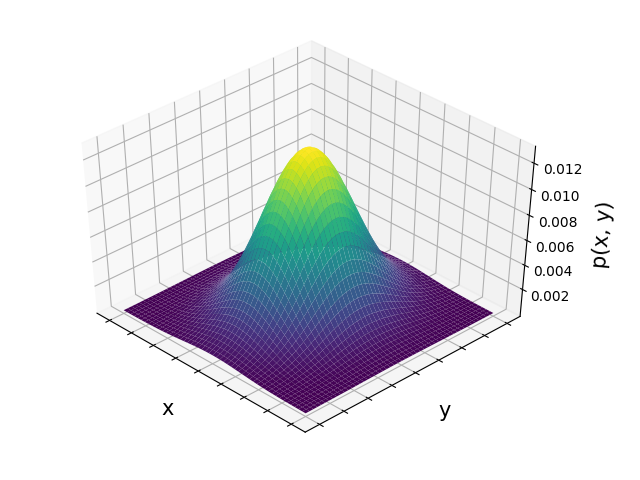
\includegraphics[width=\textwidth]{gauss-bivariate}
        \caption{Normalna porazdelitev v dveh dimenzijah.}
    \end{figure}
\end{zgled}

Izpustimo definicije in ostale primere porazdelitev, poglejmo raje, kako definiramo divergenco.
\pagebreak
Definicija divergence za bi- in multivariate porazdelitve sovpada z definicijo divergence za univariatne porazdelitve:
\begin{enumerate}
	\item $D(p \| q) \geq 0$ za vsaka $p, q \in S$, kjer je $S$ množica porazdelitev,
	\item $D(p \| q) = 0 \Leftrightarrow p = q$.
\end{enumerate}

Recimo, da gledamo porazdelitve v $n$ dimenzijah. Gostote verjetnosti teh porazdelitev bodo funkcije $p: \Omega \subseteq \RR^n \rightarrow \RR^+$. Divergence se torej na naraven način prevedejo za $n$-dimenzionalne porazdelitve. Poglejmo si to na primerih.

\begin{zgled}
    Naj bo $x=(x_1, x_2, \dots , x_n) \in \RR^n$. Naj bodo $p, q$ gostote verjetnosti z definicijskim območjem $\Omega \subseteq \RR^n$. Definicije divergenc razširimo na $n$ dimenzij:
	\begin{enumerate}
		\item \textbf{Kullback-Leiblerjeva divergenca}
		\begin{equation}
			D_{KL}(p \| q) = \idotsint\limits_\Omega p(x) \cdot \log\Big(\frac{p(x)}{q(x)}\Big) \  dx_1\dots dx_n.
		\end{equation}
		\item \textbf{f-divergenca}
		\begin{equation}
			D_f(p \| q) = \idotsint\limits_\Omega p(x) \cdot f\Big(\frac{p(x)}{q(x)}\Big) \  dx_1\dots dx_n.
		\end{equation}
		\item \textbf{Hellingerjeva distanca}
		\begin{equation}
			H^2(p, q) = 2 \cdot \idotsint\limits_\Omega \Big(\sqrt{p(x)} - \sqrt{q(x)}\Big)^2 \  dx_1\dots dx_n.
		\end{equation}
		\item \textbf{Renyi divergenca}
		\begin{equation}
			D_{\alpha}(p \| q)=\frac{1}{\alpha-1} \cdot \log \Bigg(\idotsint\limits_\Omega \Big(p(x)\Big)^{\alpha}\Big(q(x)\Big)^{1-\alpha}\  dx_1\dots dx_n\Bigg), \quad \quad \alpha \neq 1.
		\end{equation}
	\end{enumerate}
\end{zgled}

\subsection{Praktična uporaba}

Divergenca glede na gostoto verjetnosti je zelo uporabna v praktičnih problemih, ko glede na set podatkov naredimo oceno gostote verjetnosti z Gaussovimi jedri (angl. Gaussian kernel density estimation).

V splošnem bomo hoteli izračunati divergenco med dvema statističnima vzorcema. Skoraj nikoli divergence ne računamo analitično, saj pri obdelavi podatkov nimamo podane gostote verjetnosti teh podatkov eksplicitno in simbolno. Divergenco bomo izračunali z uporabo histogramov vzorcev ali pa z uporabo ocenjevalcev za gostoto verjetnosti.